\documentclass[a4paper]{beamer}
\usepackage{beamerthemePadovaDEI}

\usepackage[utf8]{inputenc}
\usepackage[T1]{fontenc}
\usepackage{mathtools}
\usepackage{lmodern}
\usepackage{textcomp}
\usepackage{subcaption}
\captionsetup{compatibility=false}
\usepackage[italian]{babel}
\usepackage{multirow}
\usepackage{array,booktabs,ragged2e}
\newcolumntype{R}[1]{>{\RaggedLeft\arraybackslash}p{#1}}

\title[title]{Esperimenti MIP per una classe di\\problemi di assegnamento quadratico}
\author[Persone]{Laureando: Mattia Toffolon\\Relatore: Prof. Domenico Salvagnin}
\date{\small \textit{Padova, 18 luglio 2023}}

\begin{document}
%
%% title
\begin{frame}
\maketitle
\end{frame}

\begin{frame}{Indice}
	\begin{itemize}
		\item Introduzione al problema di assegnamento quadratico
		\vfill
		\item Istanze Tai*c
		\vfill
		\item Modellazione algebrica
		\vfill
		\item Risultati sperimentali
		\vfill
		\item Conclusioni
		\vfill
	\end{itemize}
\end{frame}

\begin{frame}{Quadratic assignment problem}
Il problema di ottimizzazione di assegnamento quadratico (QAP) consiste nell'assegnare \textbf{\textit{n} unità} in 
\textbf{\textit{n} posizioni} differenti. 

Sono noti il flusso di informazioni da trasferire da ogni unità alle altre
e per ogni coppia di posizioni la distanza che le separa.
\newline \newline
L'assegnamento ottimale è quello che rende \textbf{minima} la \textbf{somma dei prodotti flusso x distanza} relativi ad ogni coppia
di unità.
\newline \newline
Matematicamente, il problema può essere espresso come segue
\begin{align*}
    \min_{\pi \, \in \, P(n)} \sum_{i\,=\,1}^{n} \sum_{j=1}^{n} a_{ij} b_{\pi_{i} \pi_{j}}
\end{align*}
\end{frame}

\begin{frame}{Istanze Tai*c}
La classe di problemi QAP studiata è quella delle istanze \textbf{Tai*c}.
\newline \newline
Tali istanze sono generate dal metodo \textbf{\textit{Densità di grigio}}.
Questo si fonda sull'uso di un'apposita griglia composta da \textit{n} caselle ed un valore di densità per ottenere i parametri 
di distanza e flusso.
\newline \newline
Le soluzioni a queste istanze possono essere visulizzate come griglie e combinate per ottenere la tonalità di grigio desiderata.
\begin{figure}[h!]
    \centering
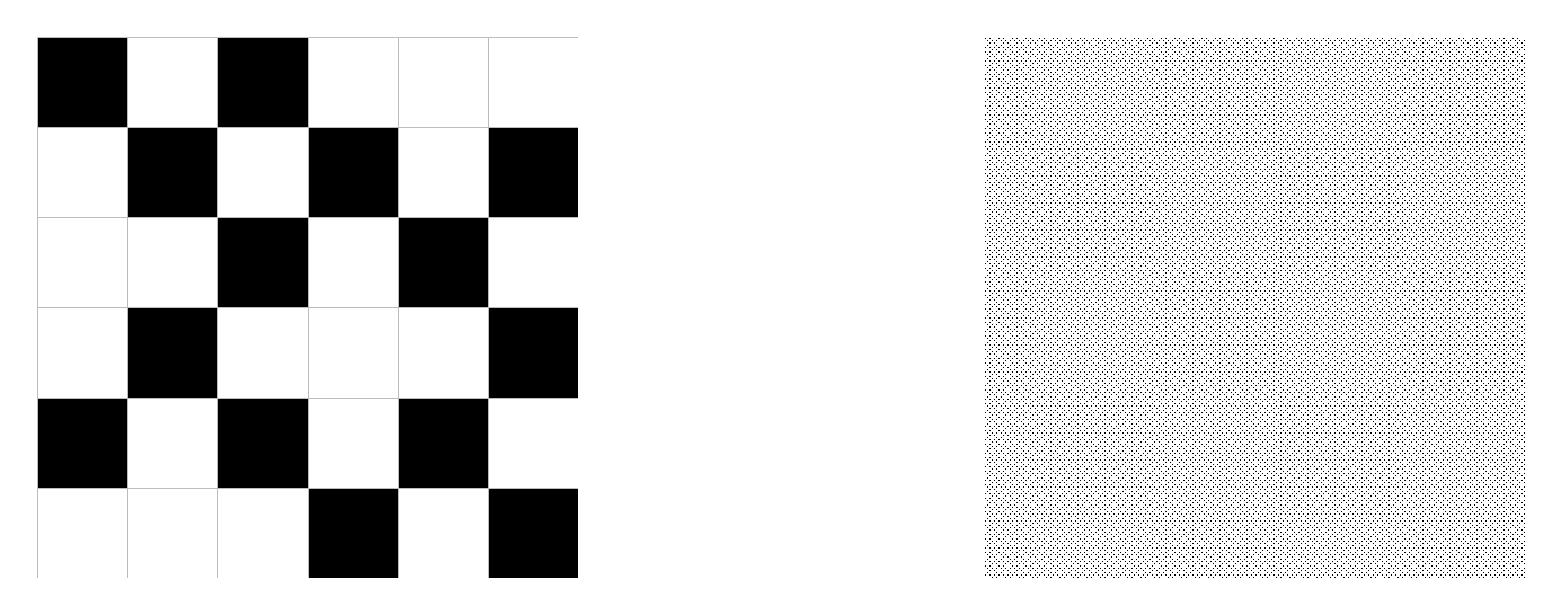
\includegraphics[scale=0.12]{images/gray_36_40.png}
\caption{Esempio per un'istanza di dimensione 36 a densità 40\%}
\end{figure}   
\end{frame}

\begin{frame}{Modellazione algebrica - 1}
Le diverse fasi in cui si è articolata la modellazione algebrica del problema di ottimizzazione sono state:
\begin{itemize}
\item individuazione degli insiemi
\item individuazione dei parametri
\item individuazione delle variabili
\item definizione dei vincoli e della funzione obiettivo
\item linearizzazione del modello 
\item semplificazione del modello
\end{itemize}
\vfill
Le ultime due fasi sono state necessarie per adattare il modello alla \textbf{forma MIP} e per \textbf{ridurre il costo computazionale}
richiesto per risolvere le verie istanze del problema.
\end{frame}

\begin{frame}{Modellazione algebrica - 2}
Il risultato dalla modellazione algebrica è il seguente modello:
\begin{align*}
	\begin{array}{l}
      \min \, \sum_{i\in I} \sum_{j\in I} \, b_{ij}\cdot y_{ij} \\
      \sum_{i\in I} \, x_{i} = n_1 \\
      y_{ij} \, \leq \, x_{i}   \;\;\;\qquad \forall \; i,j \in I \\ 
      y_{ij} \, \leq \, x_{j}   \;\;\;\qquad \forall \; i,j \in I \\
      y_{ij} \, \geq \, x_{i} + x_{j} - 1      \,\qquad \forall \; i,j \in I\\
      x_{i} ,\, y_{ij} \in \{0,1\}      \;\quad\qquad \forall \; i,j \in I
    \end{array}
\end{align*}
\vfill
Si nota come, dato \textit{n} il numero di unità e di posizioni, è necessario prendere in esame \textbf{\textit{n}$^{\textbf{2}}$ variabili}. 
Da qui deriva l'elevata complessità di risoluzione delle istanze del problema in oggetto.
\end{frame}

\begin{frame}{Risultati sperimentali - 1}
Tramite alcuni script \textit{Python} ed il software risolutore \textit{CPLEX} è stato possibile trovare le soluzioni ad alcune istanze del problema
e ricavare i \textbf{tempi medi di risoluzione} riportati nella seguente tabella.
\begin{tabular}{c R{1cm}|R{1cm}|R{1cm}|R{1cm}|R{1cm}|R{1cm}|R{1cm}| l}
    \centering
    & \multicolumn{6}{ c }{} \\ \cline{3-8}
    & & \multicolumn{1}{ c| }{9} & 16 \hphantom{n} & 25 \hphantom{n} & 36 \hphantom{n} & 42 \hphantom{n} & 45 \hphantom{n} & \\ \cline{2-8}
    \multicolumn{1}{  c  }{} &
    \multicolumn{1}{ |c| }{10\%} & 0.2 & 0.1 & 0.3 & 0.6 & 0.8 & 1.1  &  \\ \cline{2-8}
    \multicolumn{1}{  c  }{}                       &
    \multicolumn{1}{ |c| }{20\%} & 0.1 & 0.1 & 0.3 & 0.9 & 5.0 & 13.0 &   \\ \cline{2-8}
    \multicolumn{1}{  c  }{}                       &
    \multicolumn{1}{ |c| }{30\%} & 0.1 & 0.1 & 0.3 & 13.0 & 296.4 & 913.0 &   \\ \cline{2-8}
    \multicolumn{1}{  c  }{}                       &
    \multicolumn{1}{ |c| }{40\%} & 0.1 & 0.2 & 1.6 & 66.9 & 1611.0 & 4896.7 &   \\ \cline{2-8}
    \multicolumn{1}{  c  }{} &
    \multicolumn{1}{ |c| }{50\%} & 0.1 & 0.2 & 2.6 & 18.4 & 373.0 & 2942.4 &   \\ \cline{2-8}
    \multicolumn{1}{  c  }{}                       &
    \multicolumn{1}{ |c| }{60\%} & 0.1 & 0.2 & 2.5 & 97.7 & 2209.5 & 6708.0 &   \\ \cline{2-8}
    \multicolumn{1}{  c  }{}                       &
    \multicolumn{1}{ |c| }{70\%} & 0.1 & 0.1 & 0.7 & 70.8 & 1641.5 & 5853.2 &   \\ \cline{2-8}
    \multicolumn{1}{  c  }{}                       &
    \multicolumn{1}{ |c| }{80\%} & 0.1 & 0.1 & 0.5 & 6.4 & 36.4 & 158.7 &   \\ \cline{2-8}
    \multicolumn{1}{  c  }{}                       &
    \multicolumn{1}{ |c| }{90\%} & 0.1 & 0.1 & 0.3 & 0.8 & 1.3 & 5.7 &    \\ \cline{2-8}
    \medskip
\end{tabular}
\end{frame}

\begin{frame}{Risultati sperimentali - 2}
	I dati ottenuti dalle sperimentazioni sono stati utilizzati per tracciare i seguenti grafici. Essi rappresentano
	l'andamento dei tempi rispetto alla dimensione dell'istanza e alla densità di grigio.
	\begin{figure}[h!]
		\centering
		\begin{subfigure}[b]{0.41\textwidth}
			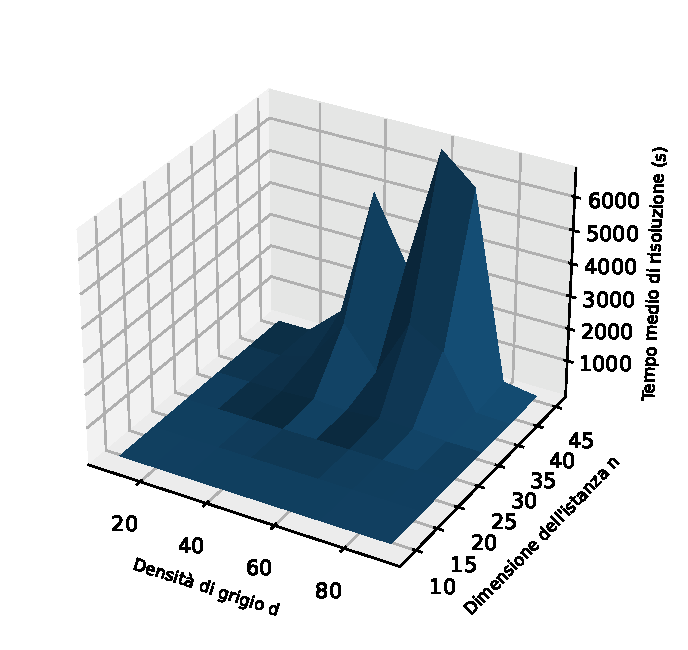
\includegraphics[width=\textwidth]{images/resolution_times.eps}
			\caption{Grafico 3D}
		\end{subfigure}
		\hspace{2em}
		\begin{subfigure}[b]{0.49\textwidth}
			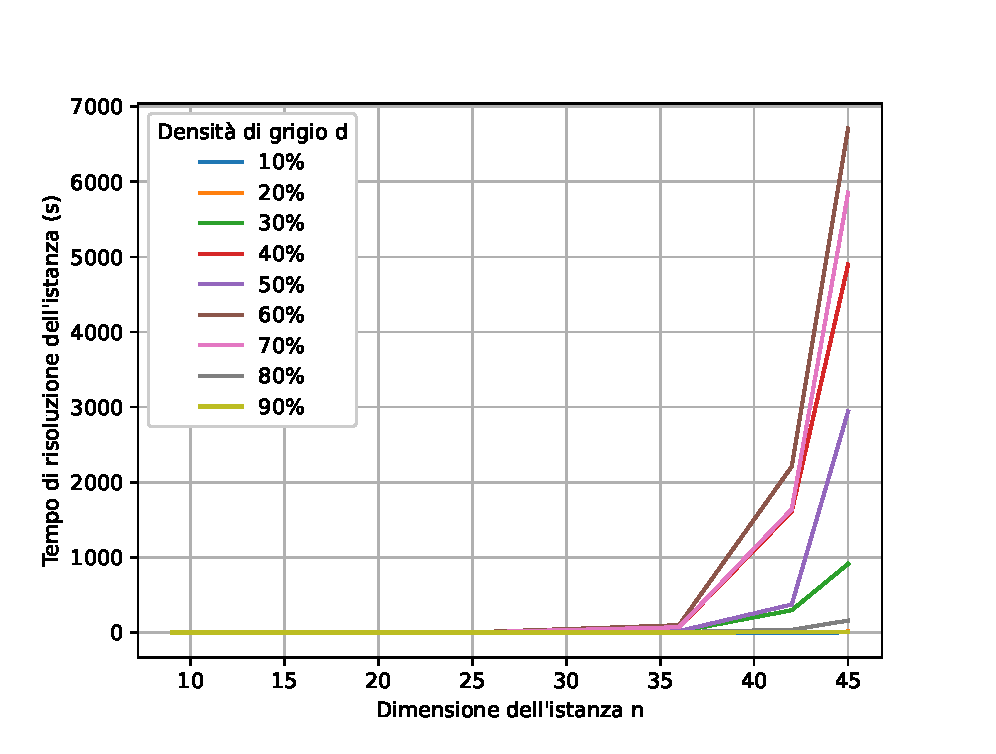
\includegraphics[width=\textwidth]{images/resolution_times2.eps}
			\caption{Grafico 2D}
		\end{subfigure}
	\end{figure}
\end{frame}

%\begin{frame}{Risultati sperimentali - 2}
%Dai grafici è possibile osservare una correlazione di tipo \textbf{esponenziale} tra il tempo medio di risoluzione e la dimensione dell'istanza
%per ogni valore di densità preso in esame.
%\newline \newline
%L'unica differenza tra i diversi casi consiste nella velocità con cui i valori dei tempi divergono. Per densità prossime al 50\% il fenomeno è più marcato, 
%mentre per quelle vicine allo 0\% o al 100\% esso tende ad essere più fievole.
%\newline \newline 
%Tali risultati risultano compatibili con le ipotesi formulabili limitandosi ad osservare le teoria.
%\end{frame}

\begin{frame}{Risultati sperimentali - 3}
Le soluzioni ottime delle istanze possono essere visulizzate come griglie "densità di grigio".
Quelle qui riportate corrispondono alle soluzioni trovate per tre istanze differenti.
\vfill
\begin{figure}[h!]
    \centering
    \begin{subfigure}[b]{\textwidth}
        \centering
        \begin{subfigure}[b]{0.25\textwidth}
            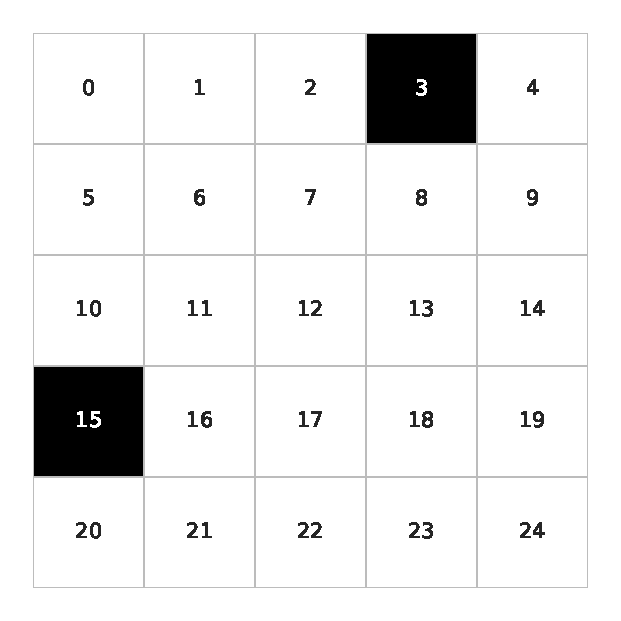
\includegraphics[width=\columnwidth]{images/Tai25c_5x5_10.eps}
			\caption{n=25 d=10\%}
        \end{subfigure}
        \hspace{1em}
        \begin{subfigure}[b]{0.25\textwidth}
            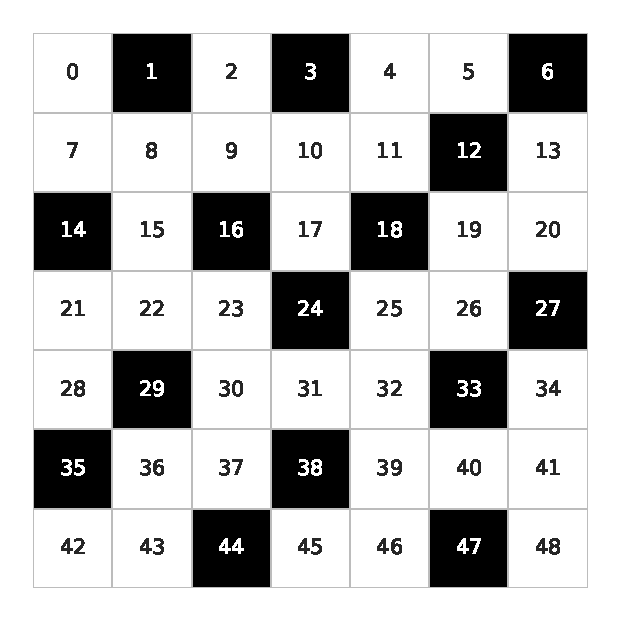
\includegraphics[width=\columnwidth]{images/Tai49c_7x7_30.eps}
			\caption{n=49 d=30\%}
        \end{subfigure}
        \hspace{1em}
        \begin{subfigure}[b]{0.25\textwidth}
            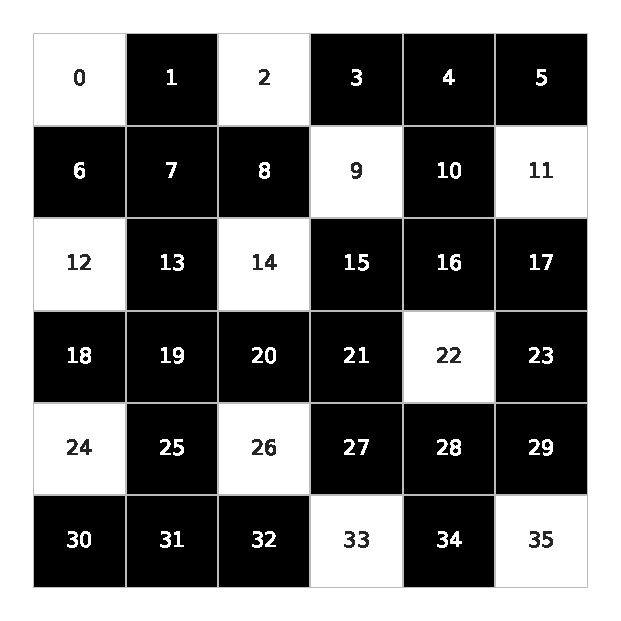
\includegraphics[width=\columnwidth]{images/Tai36c_6x6_70.eps}
			\caption{n=36 d=70\%}
        \end{subfigure}
     \end{subfigure}
\end{figure}
\end{frame}

\begin{frame}{Conclusioni}
\textbf{Risultati}\\
\begin{itemize}
\item L'andamento dei tempi medi di risoluzione rispetto alla dimensione dell'istanza è generalmente esponenziale. \newline Al variare del valore di densità si notano differenze minori.
\item Tramite la visualizzazione per griglie si può confermare la validità delle soluzioni rispetto al metodo di generazione.
\end{itemize}
\vfill
\textbf{Possibili futuri sviluppi}\\
\begin{itemize}
\item estensione del time limit imposto al risolutore CPLEX 
\item utilizzo di un calcolatore più potente per risolvere istanze di dimensioni maggiori
\item ricerca di un modello più efficiente
\end{itemize}
\end{frame}

\begin{frame}{Ringraziamenti}
\centering
\LARGE Grazie per l'attenzione!
\end{frame}

\begin{frame}
\maketitle
\end{frame}

\end{document}